\documentclass{article}
\usepackage{graphicx}
\usepackage[rightcaption]{sidecap}
\graphicspath{ {./billeder/} }
\usepackage{amsmath,amsfonts,stmaryrd,amssymb}
\usepackage[ruled]{algorithm2e}
\usepackage[framemethod=tikz]{mdframed}
\usepackage{parskip}
\usepackage{nameref}
\usepackage{booktabs}
\usepackage{tabularx}
\usepackage{geometry}
\geometry{
	paper=a4paper,
	top=2.5cm,
	bottom=3cm,
	left=2.5cm,
	right=2.5cm,
	headheight=14pt,
	footskip=1.5cm,
	headsep=1.2cm,
	%showframe, % Uncomment to show how the type block is set on the page
}

\usepackage[utf8]{inputenc}
\usepackage[T1]{fontenc}
\usepackage{XCharter}
\usepackage{graphicx}

\author {Jesper Toplund}
\title{Roadmap for komponenter}
\date{}

\begin{document}
\maketitle

\vspace{20 mm}
\begin{quote}
    \textit{}
\end{quote}
\newpage{}
\clearpage

\section{Baggrund}
\subsection{Formål}

% \subsection{Datagrundlag}
% Denne sektion kan udelades.

\subsection{Omfang}

\section{Generelt forarbejde}
\subsection{Indholds datamodel}
Noget af det vigtigste for at få arkitekturen til at hænge sammen er at vi får etableret en generel og gennemgående datamodel, som kan være med til at sikre at alle vores komponenter kan kommunikere på tværs. Det er et vigtigt stykke forarbejde som både bidrager til muligheden for at rydde op i den hårknude som arkitekturen er nu og gør det muligt at sikre at nyudviklede komponenter kan benyttes på tværs. Det kommer til at kræve en del arbejde at få etableret denne datamodel og derefter at få de forskellige systemer tilpasset til denne datamodel.

Det anbefales at vi starter med at udarbejde en så dækkende model som muligt, gerne en der læner sig op ad den som allerede benyttes af Steffi. Dermed får vi et centralt udgangspunkt som, når det bredes ud, kan bruges som samlingspunkt om vores content aggregation service.
%TODO estimater
\subsection{URN / URL}
Hvis vi samtidigt med opdateringen af datamodellen også kikker på DR URN, så kan vi sikre at det er muligt at unikt identificere indhold på tværs af systemer uden kendskab til systemlandskabet.
%TODO Der mangler helt sikkert info her 
\subsection{Underliggende infrastruktur}
\subsection{DevOps kulturen styrkes}


\section{Analyse af komponenter}

\subsection{Akamai}
\begin{figure}[h]
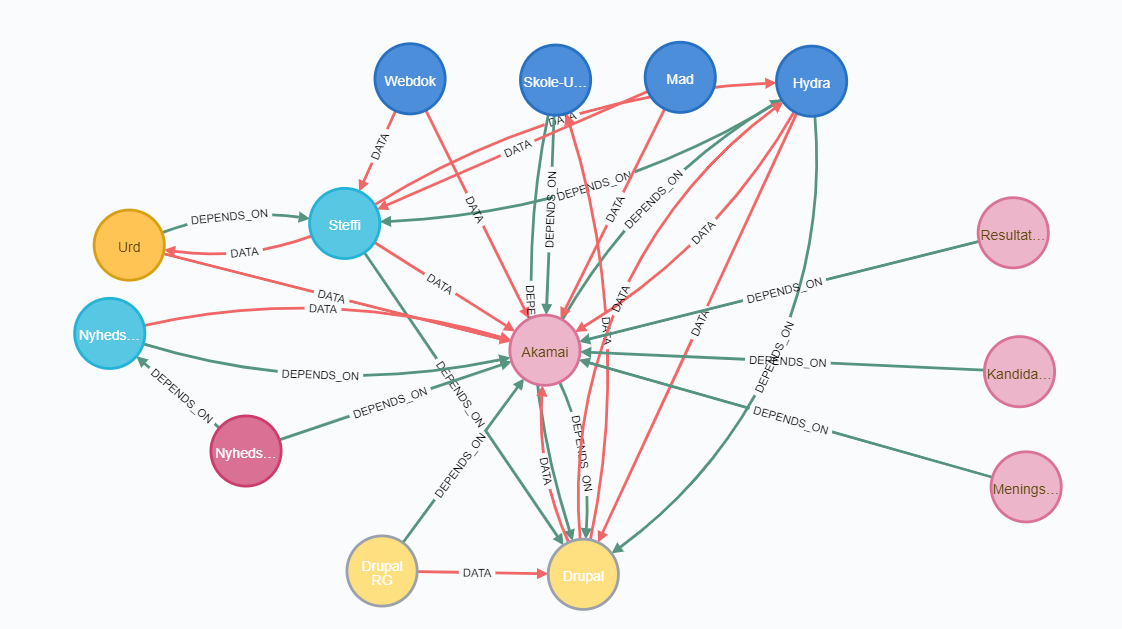
\includegraphics[width=300pt]{Akamai.PNG}
\caption{MATCH (x\{name:'Akamai'\})- -(y) RETURN x,y}
\end{figure}
\subsubsection{Kort beskrivelse}
Akamai benyttes som det primære CDN (content delivery Network). 
Det er dermed ikke et produkt som er udviklet hverken af eller for DR, 
men et produkt som vi er afhængige af. 
\subsubsection{Anbefalet handling}
Akamai som CDN udfylder fint de behov som DR har. 

Vi kan med fordel kikke på om vi benytter fornuftige cache timeouts eller om vores hjemmeside er struktureret til at få mest muligt ud af CDN.
\subsubsection{Overslag}
Indgår ikke som sådan i roadmap.



\subsection{Hydra}
\begin{figure}[h]
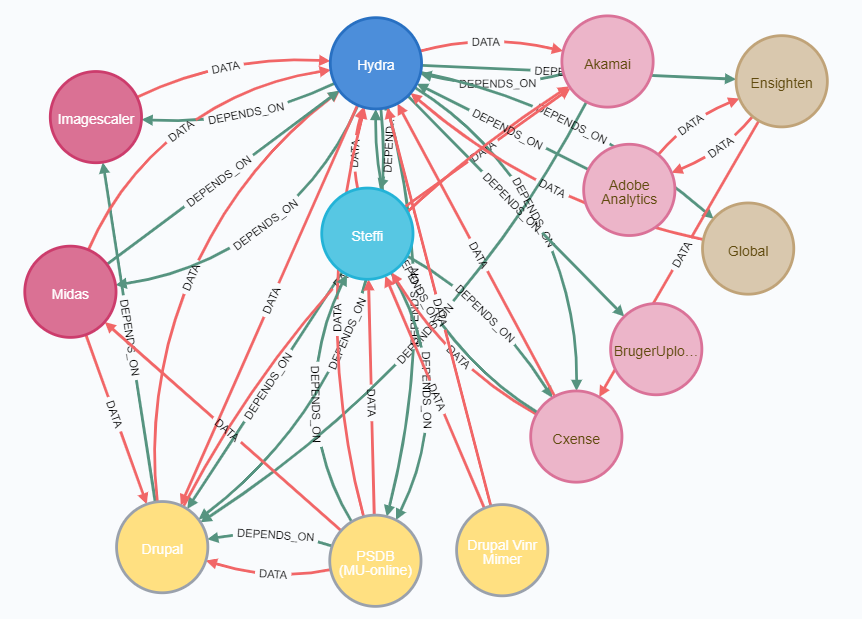
\includegraphics[width=300pt]{Hydra.PNG}
\caption{MATCH (x\{name:'Hydra'\})- -(y) RETURN x,y}
\end{figure}
\subsubsection{Kort beskrivelse}
Web-frontend, der varetager indholdsvisning for artikler og forsider. Anvender Drupal-visning til sider, der endnu ikke understøttes af Hydra.
Ovenstående figur viser at der er et højt antal afhængigheder til mange systemer. Det skal undersøges nærmere om de alle er aktuelle.
\subsubsection{Anbefalet handling}
Hydra er beskrevet som at den direkte henter data fra og sender data til Drupal. Er det korrekt, så springer den flere lag over i referencearkitekturen.
Hydra burde kun afhænge af platform utilities, platform services, product services eller content aggregation.
% TODO Verificer at alle de beskrevne afhængigheder også er aktuelle afhængigheder.
\subsubsection{Overslag}
Afklaring nødvendigt før det kan estimeres.


\subsection{Steffi}
\begin{figure}[h]
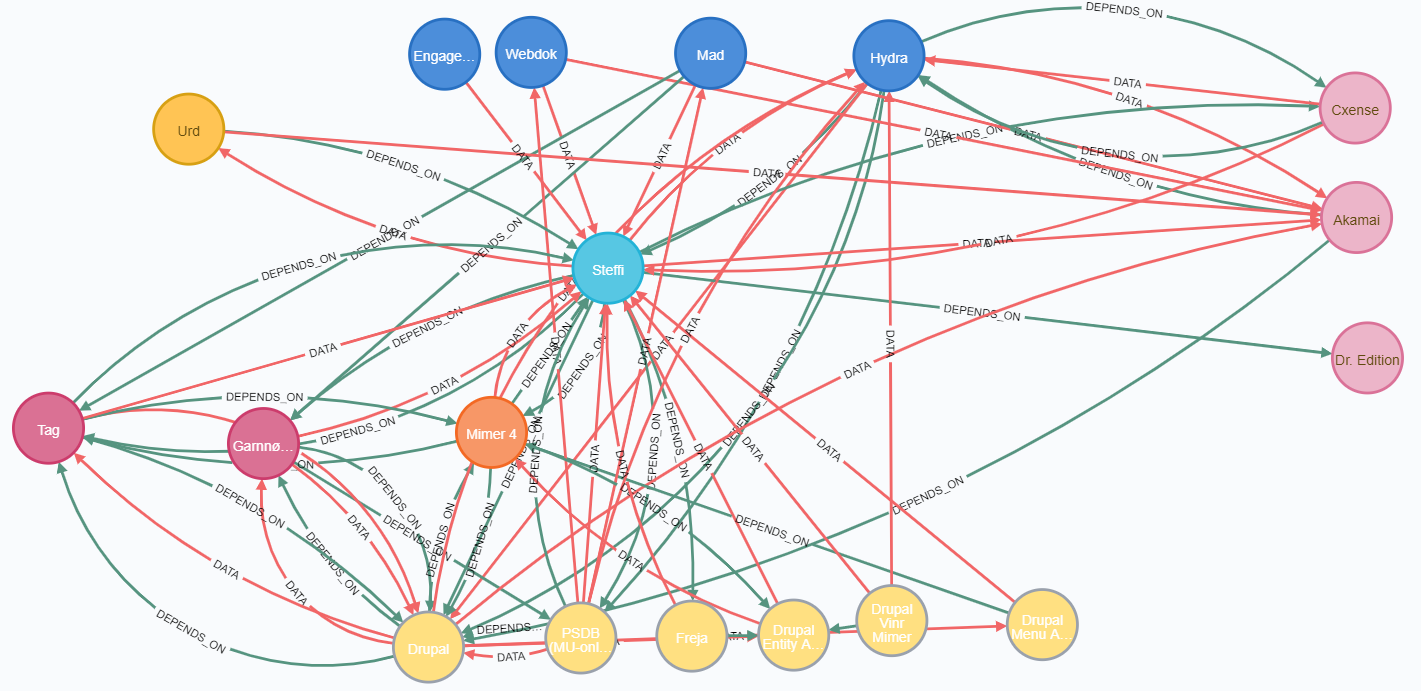
\includegraphics[width=300pt]{Steffi.PNG}
\caption{MATCH (x\{name:'Steffi'\})- -(y) RETURN x,y}
\end{figure}
\subsubsection{Kort beskrivelse}
Forespørgselslag, der tilbyder GraphQL-grænseflader til frontendapplikationer.
benyttes Content aggregering.
\subsubsection{Anbefalet handling}
\subsubsection{Overslag}


\subsection{Talentholdet}
\begin{figure}[h]
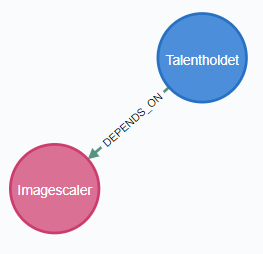
\includegraphics[width=300pt]{Talentholdet.PNG}
\caption{MATCH (x\{name:'Talentholdet'\})- -(y) RETURN x,y}
\end{figure}
\subsubsection{Kort beskrivelse}
Talentholdet er en rekrutteringsplatform for nye talenter til DR. Talentholdet har sin egen database hvori den gemmer personidentificerbar data i krypteret form. Talentholdet afhænger af Imagescaler
\subsubsection{Anbefalet handling}
Talentholdet udfører en mindre opgave som det er muligt at diskutere værdien af. Vi bør få afklaret med forretningen om vi eventuelt kan pensionere programmet. Der er en del kodegæld i programmet og GDPR sletninger er en manuel process.
Prioriteten af Talentholdet er dog ret lav, så den manuelle process kan tolereres.
\subsubsection{Overslag}
N/A

\subsection{Elements}
\begin{figure}[h]
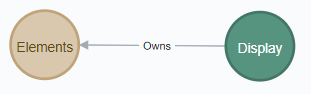
\includegraphics[width=200pt]{Elements.PNG}
\caption{MATCH (x\{name:'Elements'\})- -(y) RETURN x,y}
\end{figure}
\subsubsection{Kort beskrivelse}
Elements er DR's centrale komponentbibliotek, som består af FE komponenter. Elements er kodet i React. Elements benyttes af en række af vores Frontend products.
\subsubsection{Anbefalet handling}
Elements benyttes en række af vores Frontend products og passer fint ind i vores reference arkitektur
\subsubsection{Overslag}
N/A

\subsection{Webdok}
\begin{figure}[h]
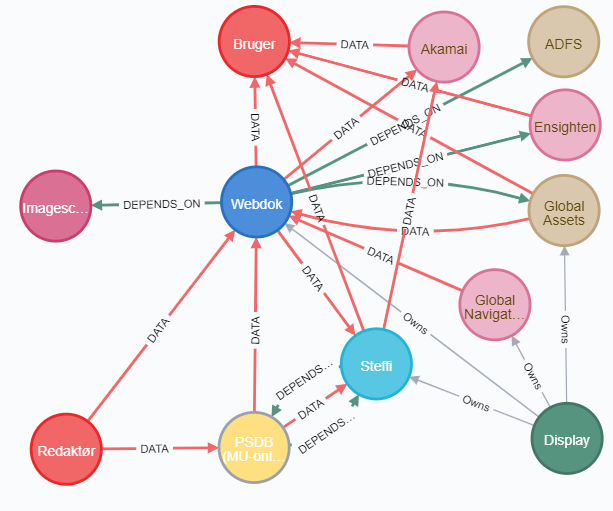
\includegraphics[width=300pt]{Webdok.PNG}
\caption{MATCH (x\{name:'Webdok'\})- -(y) RETURN x,y}
\end{figure}
\subsubsection{Kort beskrivelse}
CMS og præsentation af featureartikler i særformater.	
Præsentationslag (Node.js) trækker data fra API (.NET). Redaktørgrænseflade er bygget ind i præsentationslaget.
\subsubsection{Anbefalet handling}
Hvordan Webdok er flettet ind i vores nuværende arkitektur skal undersøges nærmere. Dokumentationen som den står nu giver et lidt mudret billede
% TODO
\subsubsection{Overslag}
Ukendt.
\newpage{}
\clearpage


\subsection{Skole-Undervisning}
\begin{figure}[h]
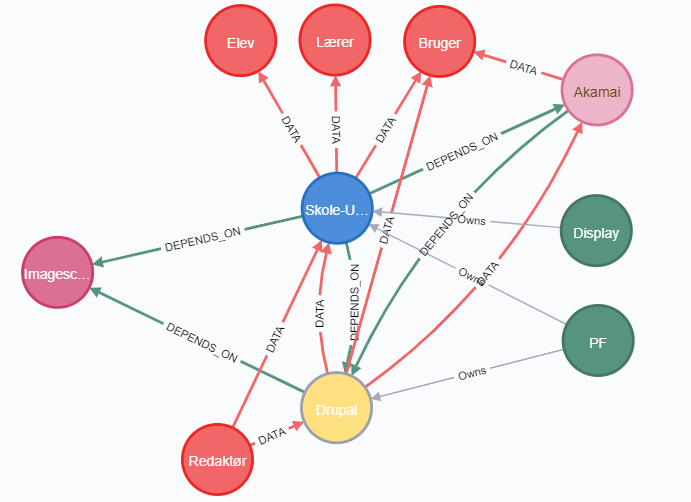
\includegraphics[width=300pt]{Skole-Undervisning.PNG}
\caption{MATCH (x\{name:'Skole-Undervisning'\})- -(y) RETURN x,y}
\end{figure}
\subsubsection{Kort beskrivelse}
Skole og Undervisning er et site, der formidler undervisningsforløb og undervisningsmateriale til Skoler.  Sitet er opbygget i Drupal, men har en række specialløsninger konstrueret for at kunne samle temaer og autogenerere faktabokse etc. 
\subsubsection{Anbefalet handling}
Skole-Undervisning passer ikke ind i referencearkitekturen, idet den udgør sin helt egen silo og udstiller data direkte til slutbrugere via Akamai. 
Afhængigt af levetiden for projektet (gartner Time model) skal vi overveje hvad vi gør ved projektet.
\subsubsection{Overslag}
Afklaring mangler.
%TODO

\subsection{Mad}
\begin{figure}[h]
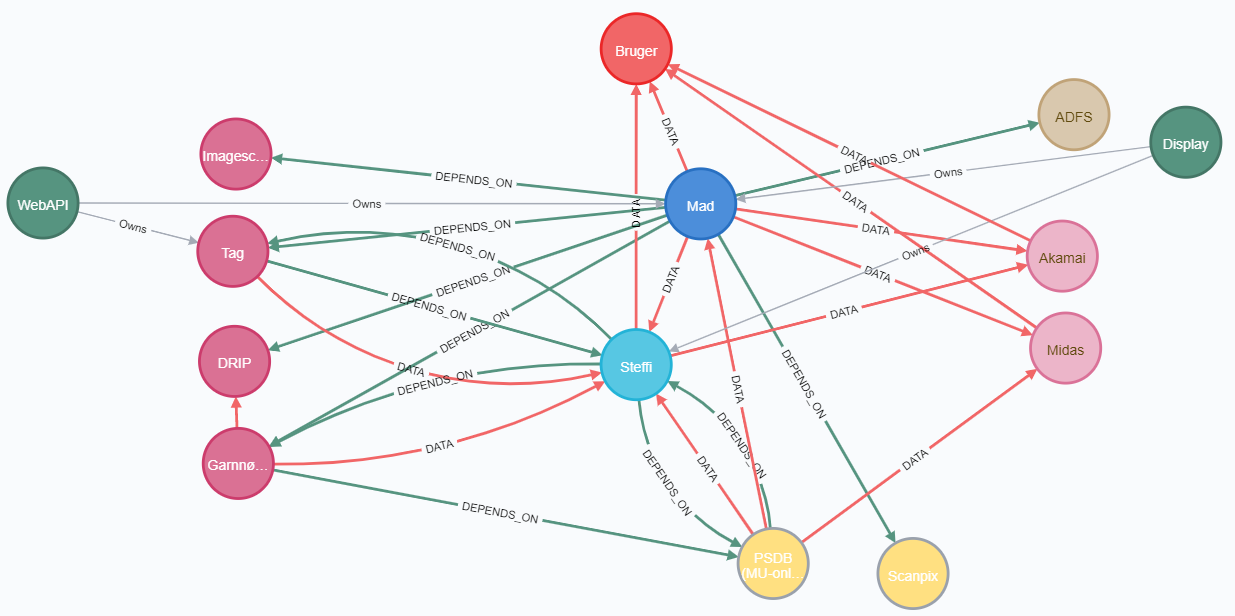
\includegraphics[width=300pt]{Mad.PNG}
\caption{MATCH (x\{name:'Mad'\})- -(y) RETURN x,y}
\end{figure}
\subsubsection{Kort beskrivelse}
Mad er en applikation, der håndterer opskrifter, artikler og opskriftssamlinger. Mad er bygget som Headless Drupal med egen RG til opskrifter. Artikler publiceres gennem Drupal. 
\subsubsection{Anbefalet handling}
Mad passer ikke helt ind i referencearkitekturen som beskrevet. Om det er en mangel i dokumentationen eller i arkitekturen skal undersøges. (hvorfor tilgår Steffi Mad direkte og ikke igennem f.eks. Mimer?)
\subsubsection{Overslag}
Afklaring mangler
%TODO

\subsection{Nyhedsapp-Frontend}
\begin{figure}[h]
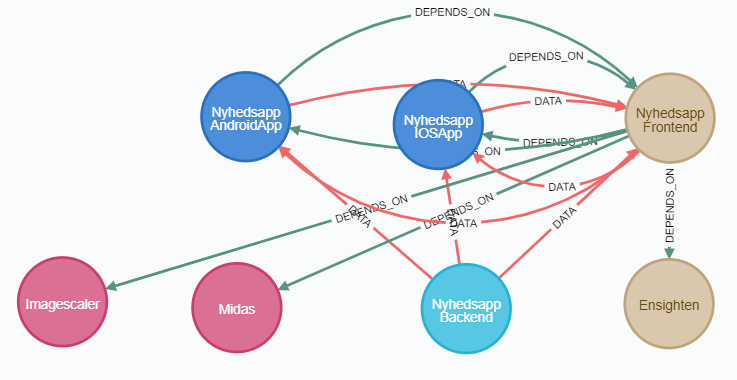
\includegraphics[width=300pt]{Nyhedsapp-Frontend.PNG}
\caption{MATCH (x\{name:'Nyhedsapp Frontend'\})- -(y) RETURN x,y}
\end{figure}
\subsubsection{Kort beskrivelse}
Præsentationslag for indhold i Nyhedsapp, således at visningen mellem iOS og Android er homogen, samt har lignende homogenitet til visningen på DR.dk
Nyhedsapp-Frontend er ikke en selvstændig applikation, men et delt kodelag der anvendes af IOS og Android udgaven af nyhedsappen. 
\subsubsection{Anbefalet handling}
Nyhedsapp-Frontend er en parallel implementering i forhold til Elements. Hvis der er ændringer i visningen af en artikel der kan vises både i nyhedsapp og på web, så skal der foretages ændringer i både Elements og Nyhedsapp-Frontend. Ved en renovation af Nyhedsapp-Frontend bør det undersøges om vi kan benytte en fælles kodebase til definition af visning.
\subsubsection{Overslag}
%TODO Sammensmeltning med Elements??
N/A

\subsection{Nyhedsapp IOS}
\begin{figure}[h]
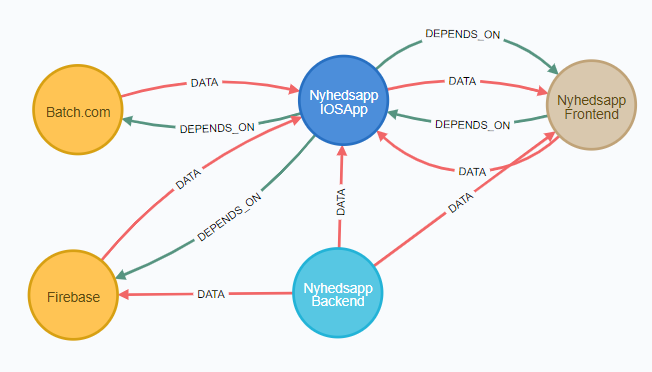
\includegraphics[width=300pt]{Nyhedsapp-IOS.PNG}
\caption{MATCH (x\{name:'Nyhedsapp IOSApp'\})- -(y) RETURN x,y}
\end{figure}
\subsubsection{Kort beskrivelse}
Afvikler Nyhedsapp Frontend, integrerer til iOS-native funktionalitet
\subsubsection{Anbefalet handling}
Nyhedsapp til både IOS og Android overholder referencearkitekturen. Der er måske ønsker om at opdatere applikationerne så de får et mere moderne udtryk på telefonerne. Dette ønske er dog et forretningsdrevet ønske og ikke en nødvendighed set ud fra reference arkitekturen
\subsubsection{Overslag}
Ingen ændringer nødvendige

\subsection{Nyhedsapp AndroidApp}
\begin{figure}[h]
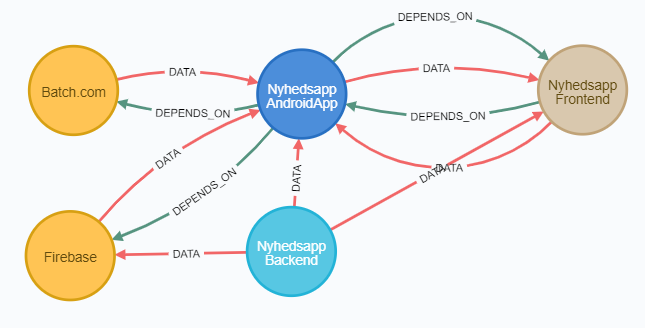
\includegraphics[width=300pt]{Nyhedsapp-Android.PNG}
\caption{MATCH (x\{name:'Nyhedsapp AndroidApp'\})- -(y) RETURN x,y}
\end{figure}
\subsubsection{Kort beskrivelse}
Native Android-wrapper, der afvikler Nyhedsapp Frontend
\subsubsection{Anbefalet handling}
Nyhedsapp til både IOS og Android overholder referencearkitekturen. Der er måske ønsker om at opdatere applikationerne så de får et mere moderne udtryk på telefonerne. Dette ønske er dog et forretningsdrevet ønske og ikke en nødvendighed set ud fra reference arkitekturen
\subsubsection{Overslag}
Ingen ændringer nødvendige


\subsection{Batch.com}
\begin{figure}[h]
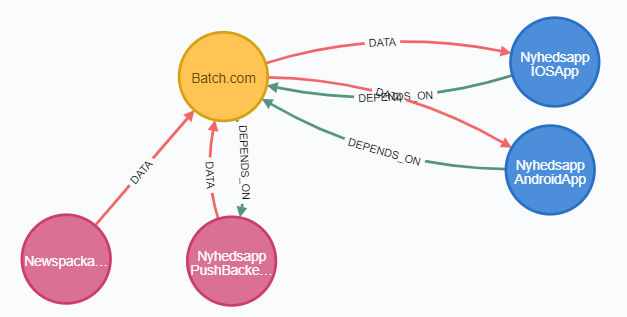
\includegraphics[width=300pt]{Batch-com.PNG}
\caption{MATCH (x\{name:'Batch.com'\})- -(y) RETURN x,y}
\end{figure}
\subsubsection{Kort beskrivelse}
SaaS tejneste der benyttes til push af beskeder til NyhedsApp
Distribuerer data til Nyhedsapp-instanser, med mulighed for dublikeringskontrol så den samme enhed kun modtager data én gang, og ligeledes en opfølgningsmulighed så devices der var utilgængelige på udsendelsestidspunktet, opdateres når de er tilgængelige igen
\subsubsection{Anbefalet handling}
Tjenesten passer ind i vores referencearkitektur. Om Batch.com bliver ved med at være den bedste løsning for push af beskeder vil vi ikke tage stilling til i dette dokument.
\subsubsection{Overslag}
Ingen ændringer nødvendige


\subsection{Firebase}
\begin{figure}[h]
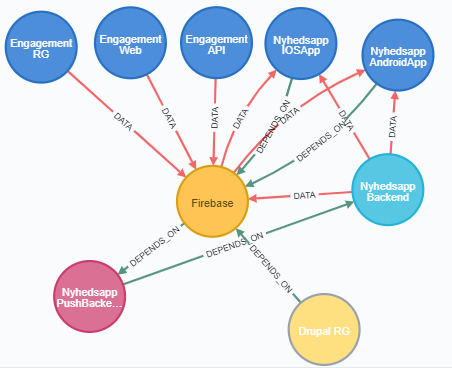
\includegraphics[width=300pt]{Firebase.PNG}
\caption{MATCH (x\{name:'Firebase'\})- -(y) RETURN x,y}
\end{figure}
\subsubsection{Kort beskrivelse}
SaaS tjeneste der benyttes til Pusg service af flere applikationer:
Nyhedsapp, Drupal RG ("hvem er inde på min artikel")
\subsubsection{Anbefalet handling}
Tjenesten passer ind i vores referencearkitektur. Om Firebase bliver ved med at være den bedste løsning for push af beskeder vil vi ikke tage stilling til i dette dokument.
\subsubsection{Overslag}
Ingen ændringer nødvendige


\subsection{OCS}
\begin{figure}[h]
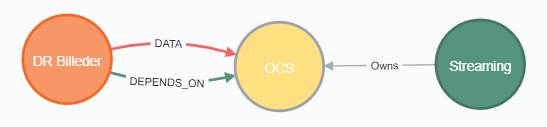
\includegraphics[width=300pt]{OCS.PNG}
\caption{MATCH (x\{name:'OCS'\})- -(y) RETURN x,y}
\end{figure}
\subsubsection{Kort beskrivelse}
API-afløseren til PSDB (MU-online), der leverer video- og radio-data (ikke anvendt i Web \& Apps endnu)	Udstiller program- og seriedata, således at aftagere kan benytte dette til at vise TV/Radio-indhold
\subsubsection{Anbefalet handling}
Ved ændringer i systemer der afhænger af PSDB, så bør det undersøges om det er relevant at anvende OCS i stedet.
\subsubsection{Overslag}
Da OCS ikke ejes af Web og Apps og da ingen systemer afhænger af OCS endnu, så er der ingen indsatser nødvendige på OCS.


\subsection{Garnnøgle}
\begin{figure}[h]
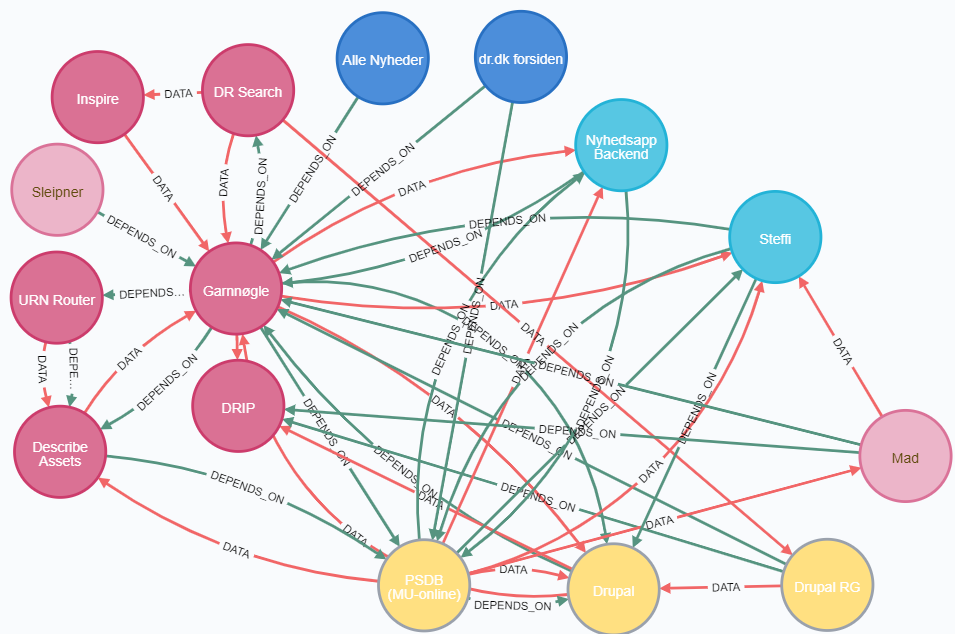
\includegraphics[width=300pt]{Garnnoegle.PNG}
\caption{MATCH (x\{name:'Garnnøgle'\})- -(y) RETURN x,y}
\end{figure}
\subsubsection{Kort beskrivelse}
Tema- og sagskategorisering af artikelindhold, således specielt nyhedsindhold kan inddeles i overordnede kategorier. Bruges også som emnebaseret abonnement-mekanisme i Nyhedsapp
Garnnøgle er ret central i værdikæden for DR.dk, da den benyttes af en lang række systemer og funktioner. Garnnøgle applikationen er behæftet med en del teknisk gæld og unødig kompleksitet i dens implementering.
\subsubsection{Anbefalet handling}
Garnnøgles placering i forhold til referencearkitekturen er ok. Selve implementeringen af garnnøgle bør dog genbesøges og afhængigt af det reelle forretningsbehov skal vi have set på en ny implementering.
\subsubsection{Overslag}
Udvikling af ny garnnøgle: Grov estimat 8 mandeuger.


\subsection{Drupal}
\begin{figure}[h]
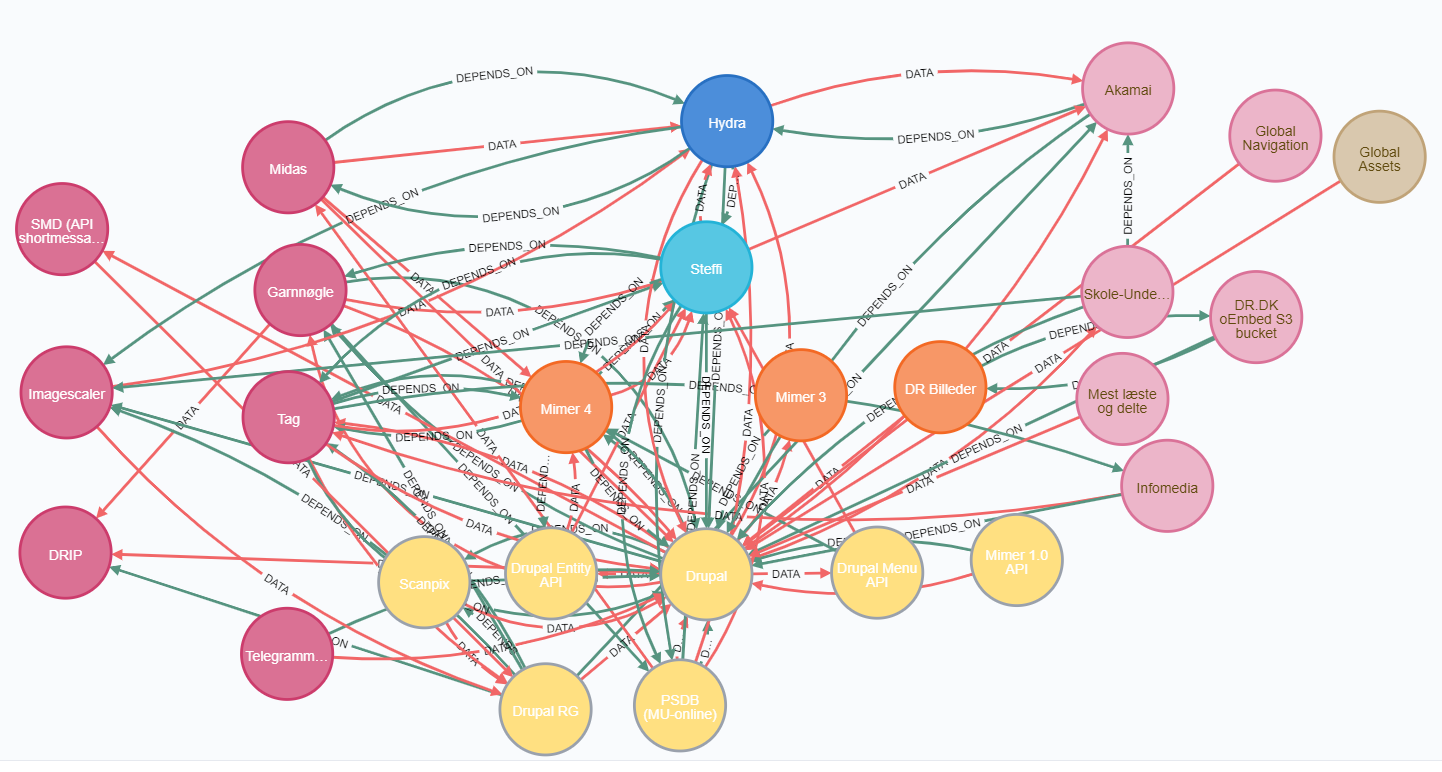
\includegraphics[width=300pt]{Drupal.PNG}
\caption{MATCH (x\{name:'Drupal'\})- -(y) RETURN x,y}
\end{figure}
\subsubsection{Kort beskrivelse}
Det primære CMS til tekstbaseret indhold på DR.dk, samt redaktionel grænseflade til indholdsproduktion og slutteligt mulighed for at grafisk opbygge sektionsforsider og sites.
\subsubsection{Anbefalet handling}
I henhold til referencearkitekturen burde Drupal kun være forbundet med Content Services og Platform Services. Da Drupal er det centrale CMS system er antallet af forbindelser ikke den store overraskelse, det peger dog entydigt på at DR stadig er meget hængt op på Drupal og dermed vil en eventuel udskiftning eller opdatering af Drupal være en stor udgift.
Vi bør helt klart se på at nedbringe antallet af direkte afhængigheder til og fra Drupal. 
Dette kan enten ske ved at lade Platform Services snakke med Content Services (f.eks. at lade garnnøgle afhænge af Mimer i stedet for Drupal), affolke og lukke de gamle udgaver af Mimer eller sikre at kun services med en god grund kan kommunikere med Drupal.

Drupal er lige nu vores styrende CMS system, det vil sige at Drupal har kontrollen med alle URL hos DR.dk, hvilket også er grunden til den direkte forbindelse fra Hydra ned til Drupal. Det vil være meget fornuftigt at kikke på at få etableret et fornuftigt URN / URL system, således at en URL / URN i sig selv er beskrivende nok til at kunne udpege det styrende indholdssystem. Det vil muliggøre sideløbende CMS systemer med hvert deres fokus og gøre det lettere at opdatere / udskifte Drupal på sigt.
 
Vi skal også have kikket på roadmap for opdatering af Drupal 7 til enten Drupal 8 eller et andet CMS system. Drupal 7 (vores nuværende installation) har end of life i november 2021.
\subsubsection{Overslag}
Migrering fra Drupal 7 til andet CMS system vil være en betydelig opgave, især med det niveau af afhængigheder og egenudvikling der er foretaget på Drupal platformen. 
Selve analysen af tidsforbrug for skiftet er uden for scope af denne rapport. Hvis vi går ud fra at det giver mening at skifte direkte fra Drupal 7 til 9 kan et groft overslag 300+ timer. Vi vil få brug for ekstern hjælp.

URN / URL 


\subsection{Mimer 1.0 API}
\begin{figure}[h]
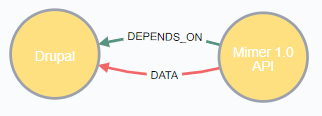
\includegraphics[width=200pt]{MimerAPI.PNG}
\caption{MATCH (x\{name:'Mimer 1.0 API'\})- -(y) RETURN x,y}
\end{figure}
\subsubsection{Kort beskrivelse}
Mimer 1.0 API er nogle REST services i Drupal, som giver Mimer 1.1 adgang til at oprette nyt indhold.
\subsubsection{Anbefalet handling}
Mimer 1.0 API er allerede under afvikling. Denne afvikling bør fortsættes og systemet lukkes.
\subsubsection{Overslag}
N/A

\subsection{Drupal RG}
\begin{figure}[h]
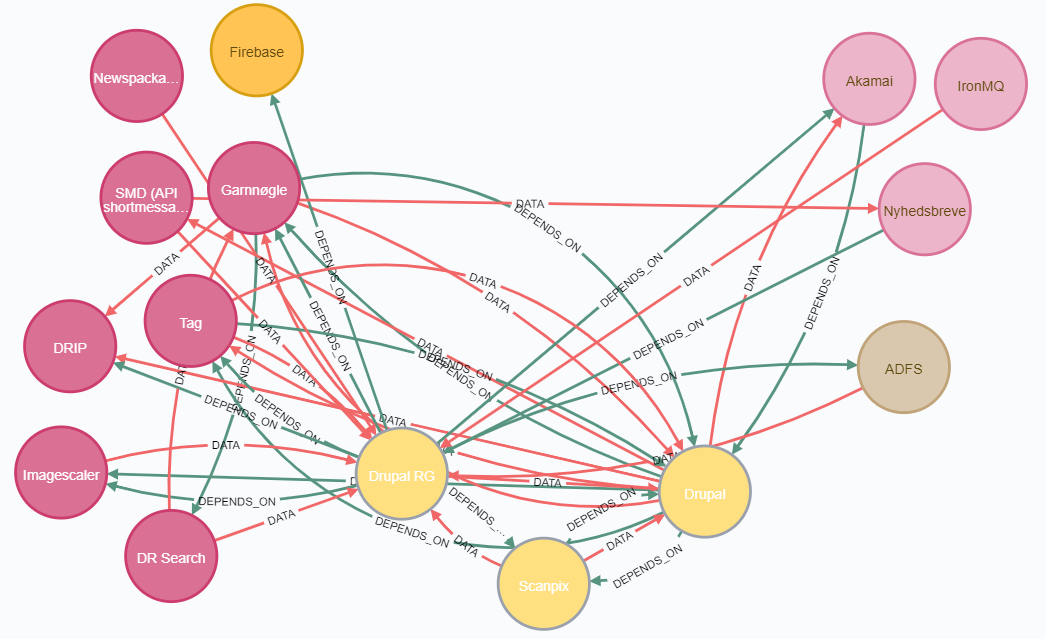
\includegraphics[width=300pt]{DrupalRG.PNG}
\caption{MATCH (x\{name:'Drupal RG'\})- -(y) RETURN x,y}
\end{figure}
\subsubsection{Kort beskrivelse}
Nyeste version af redaktør grænsefladen, lanceret Q1-2018. Redaktør grænsefladen (RG) er journalisternes værktøj til artikelproduktion. Den findes i to udgaver, hhv. RG1 og RG2.	

Webbaseret grænseflade til at oprette, redigere og distribuere tekstbaseret indhold, primært artikler. Tilbyder også integration med tema, kategoriserings, og push-funktioner.
\subsubsection{Anbefalet handling}
%TODO
\subsubsection{Overslag}


\subsection{Drupal Entity API}
\begin{figure}[h]
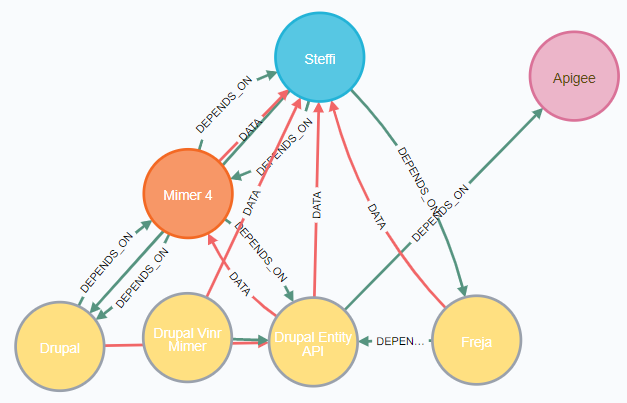
\includegraphics[width=300pt]{DrupalEntityAPI.PNG}
\caption{MATCH (x\{name:'Drupal Entity API'\})- -(y) RETURN x,y}
\end{figure}
\subsubsection{Kort beskrivelse}
Udstiller væsentlige dele af Drupals datamodel for indholdstyper i et simpelt API
\subsubsection{Anbefalet handling}
%TODO
\subsubsection{Overslag}
\newpage{}
\clearpage


\subsection{Drupal Menu API}
\begin{figure}[h]
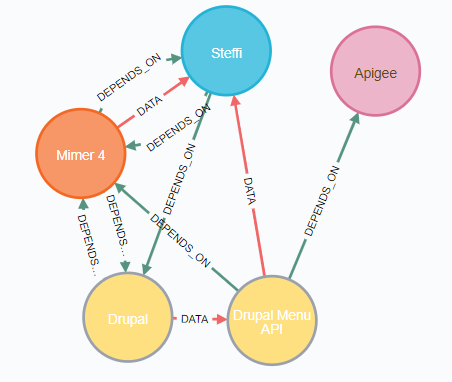
\includegraphics[width=300pt]{DrupalMenuAPI.PNG}
\caption{MATCH (x\{name:'Drupal Menu API'\})- -(y) RETURN x,y}
\end{figure}
\subsubsection{Kort beskrivelse}
Udstiller Drupals menu og sitestruktur til aftagere, der ønsker at præsentere indhold i en hierarkisk visning
\subsubsection{Anbefalet handling}
%TODO
\subsubsection{Overslag}


\subsection{Ensighten}
\begin{figure}[h]
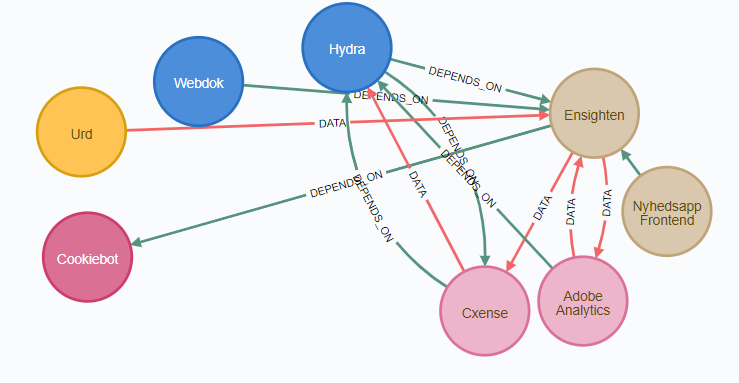
\includegraphics[width=300pt]{Ensighten.PNG}
\caption{MATCH (x\{name:'Ensighten'\})- -(y) RETURN x,y}
\end{figure}
\subsubsection{Kort beskrivelse}
Indskyder JavaScript på dr.dk sider, f.eks. til analytics, bannere, mv. Sørger derudover også for at hente og behandle metadata til analytics og anbefalingssystemer.
\subsubsection{Anbefalet handling}
\subsubsection{Overslag}


\subsection{Ad Server}
\begin{figure}[h]

\includegraphics[width=300pt]{CHANGE.PNG}
\caption{MATCH (x\{name:'CHANGE'\})- -(y) RETURN x,y}
\end{figure}
\subsubsection{Kort beskrivelse}
\subsubsection{Anbefalet handling}
\subsubsection{Overslag}


\subsection{Midas}
\begin{figure}[h]

\includegraphics[width=300pt]{CHANGE.PNG}
\caption{MATCH (x\{name:'CHANGE'\})- -(y) RETURN x,y}
\end{figure}
\subsubsection{Kort beskrivelse}
\subsubsection{Anbefalet handling}
\subsubsection{Overslag}


\subsection{PSDB (MU-online)}
\begin{figure}[h]

\includegraphics[width=300pt]{CHANGE.PNG}
\caption{MATCH (x\{name:'CHANGE'\})- -(y) RETURN x,y}
\end{figure}
\subsubsection{Kort beskrivelse}
\subsubsection{Anbefalet handling}
\subsubsection{Overslag}


\subsection{Scanpix}
\begin{figure}[h]

\includegraphics[width=300pt]{CHANGE.PNG}
\caption{MATCH (x\{name:'CHANGE'\})- -(y) RETURN x,y}
\end{figure}
\subsubsection{Kort beskrivelse}
\subsubsection{Anbefalet handling}
\subsubsection{Overslag}


\subsection{Cxense}
\begin{figure}[h]

\includegraphics[width=300pt]{CHANGE.PNG}
\caption{MATCH (x\{name:'CHANGE'\})- -(y) RETURN x,y}
\end{figure}
\subsubsection{Kort beskrivelse}
\subsubsection{Anbefalet handling}
\subsubsection{Overslag}


\subsection{Adobe Analytics}
\begin{figure}[h]

\includegraphics[width=300pt]{CHANGE.PNG}
\caption{MATCH (x\{name:'CHANGE'\})- -(y) RETURN x,y}
\end{figure}
\subsubsection{Kort beskrivelse}
\subsubsection{Anbefalet handling}
\subsubsection{Overslag}


\subsection{Pressebilleder}
\begin{figure}[h]

\includegraphics[width=300pt]{CHANGE.PNG}
\caption{MATCH (x\{name:'CHANGE'\})- -(y) RETURN x,y}
\end{figure}
\subsubsection{Kort beskrivelse}
\subsubsection{Anbefalet handling}
\subsubsection{Overslag}


\subsection{WebCMS}
\begin{figure}[h]

\includegraphics[width=300pt]{CHANGE.PNG}
\caption{MATCH (x\{name:'CHANGE'\})- -(y) RETURN x,y}
\end{figure}
\subsubsection{Kort beskrivelse}
\subsubsection{Anbefalet handling}
\subsubsection{Overslag}


\subsection{DR Search}
\begin{figure}[h]

\includegraphics[width=300pt]{CHANGE.PNG}
\caption{MATCH (x\{name:'CHANGE'\})- -(y) RETURN x,y}
\end{figure}
\subsubsection{Kort beskrivelse}
\subsubsection{Anbefalet handling}
\subsubsection{Overslag}


\subsection{Nyhedsbreve}
\begin{figure}[h]

\includegraphics[width=300pt]{CHANGE.PNG}
\caption{MATCH (x\{name:'CHANGE'\})- -(y) RETURN x,y}
\end{figure}
\subsubsection{Kort beskrivelse}
\subsubsection{Anbefalet handling}
\subsubsection{Overslag}
\newpage{}
\clearpage


\subsection{DR Billeder}
\begin{figure}[h]

\includegraphics[width=300pt]{CHANGE.PNG}
\caption{MATCH (x\{name:'CHANGE'\})- -(y) RETURN x,y}
\end{figure}
\subsubsection{Kort beskrivelse}
\subsubsection{Anbefalet handling}
\subsubsection{Overslag}


\subsection{DR.DK oEmbed S3 bucket}
\begin{figure}[h]

\includegraphics[width=300pt]{CHANGE.PNG}
\caption{MATCH (x\{name:'CHANGE'\})- -(y) RETURN x,y}
\end{figure}
\subsubsection{Kort beskrivelse}
\subsubsection{Anbefalet handling}
\subsubsection{Overslag}


\subsection{Mimer 3}
\begin{figure}[h]

\includegraphics[width=300pt]{CHANGE.PNG}
\caption{MATCH (x\{name:'CHANGE'\})- -(y) RETURN x,y}
\end{figure}
\subsubsection{Kort beskrivelse}
\subsubsection{Anbefalet handling}
\subsubsection{Overslag}


\subsection{Mimer 4}
\begin{figure}[h]

\includegraphics[width=300pt]{CHANGE.PNG}
\caption{MATCH (x\{name:'CHANGE'\})- -(y) RETURN x,y}
\end{figure}
\subsubsection{Kort beskrivelse}
\subsubsection{Anbefalet handling}
\subsubsection{Overslag}


\subsection{Tag}
\begin{figure}[h]

\includegraphics[width=300pt]{CHANGE.PNG}
\caption{MATCH (x\{name:'CHANGE'\})- -(y) RETURN x,y}
\end{figure}
\subsubsection{Kort beskrivelse}
\subsubsection{Anbefalet handling}
\subsubsection{Overslag}


\subsection{Urd}
\begin{figure}[h]

\includegraphics[width=300pt]{CHANGE.PNG}
\caption{MATCH (x\{name:'CHANGE'\})- -(y) RETURN x,y}
\end{figure}
\subsubsection{Kort beskrivelse}
\subsubsection{Anbefalet handling}
\subsubsection{Overslag}


\subsection{Infomedia}
\begin{figure}[h]

\includegraphics[width=300pt]{CHANGE.PNG}
\caption{MATCH (x\{name:'CHANGE'\})- -(y) RETURN x,y}
\end{figure}
\subsubsection{Kort beskrivelse}
\subsubsection{Anbefalet handling}
\subsubsection{Overslag}


\subsection{Auth0}
\begin{figure}[h]

\includegraphics[width=300pt]{CHANGE.PNG}
\caption{MATCH (x\{name:'CHANGE'\})- -(y) RETURN x,y}
\end{figure}
\subsubsection{Kort beskrivelse}
\subsubsection{Anbefalet handling}
\subsubsection{Overslag}


\subsection{Identity API}
\begin{figure}[h]

\includegraphics[width=300pt]{CHANGE.PNG}
\caption{MATCH (x\{name:'CHANGE'\})- -(y) RETURN x,y}
\end{figure}
\subsubsection{Kort beskrivelse}
\subsubsection{Anbefalet handling}
\subsubsection{Overslag}


\subsection{Telegrammaskine}
\begin{figure}[h]

\includegraphics[width=300pt]{CHANGE.PNG}
\caption{MATCH (x\{name:'CHANGE'\})- -(y) RETURN x,y}
\end{figure}
\subsubsection{Kort beskrivelse}
\subsubsection{Anbefalet handling}
\subsubsection{Overslag}


\subsection{Dr. Edition}
\begin{figure}[h]

\includegraphics[width=300pt]{CHANGE.PNG}
\caption{MATCH (x\{name:'CHANGE'\})- -(y) RETURN x,y}
\end{figure}
\subsubsection{Kort beskrivelse}
\subsubsection{Anbefalet handling}
\subsubsection{Overslag}


\subsection{dr.dk forsiden}
\begin{figure}[h]

\includegraphics[width=300pt]{CHANGE.PNG}
\caption{MATCH (x\{name:'CHANGE'\})- -(y) RETURN x,y}
\end{figure}
\subsubsection{Kort beskrivelse}
\subsubsection{Anbefalet handling}
\subsubsection{Overslag}


\subsection{Alle Nyheder}
\begin{figure}[h]

\includegraphics[width=300pt]{CHANGE.PNG}
\caption{MATCH (x\{name:'CHANGE'\})- -(y) RETURN x,y}
\end{figure}
\subsubsection{Kort beskrivelse}
\subsubsection{Anbefalet handling}
\subsubsection{Overslag}
\newpage{}
\clearpage


\subsection{Newsapp UI}
\begin{figure}[h]

\includegraphics[width=300pt]{CHANGE.PNG}
\caption{MATCH (x\{name:'CHANGE'\})- -(y) RETURN x,y}
\end{figure}
\subsubsection{Kort beskrivelse}
\subsubsection{Anbefalet handling}
\subsubsection{Overslag}


\subsection{SMD (API shortmessage-dispatcher)}
\begin{figure}[h]

\includegraphics[width=300pt]{CHANGE.PNG}
\caption{MATCH (x\{name:'CHANGE'\})- -(y) RETURN x,y}
\end{figure}
\subsubsection{Kort beskrivelse}
\subsubsection{Anbefalet handling}
\subsubsection{Overslag}


\subsection{Mest læste og delte}
\begin{figure}[h]

\includegraphics[width=300pt]{CHANGE.PNG}
\caption{MATCH (x\{name:'CHANGE'\})- -(y) RETURN x,y}
\end{figure}
\subsubsection{Kort beskrivelse}
\subsubsection{Anbefalet handling}
\subsubsection{Overslag}


\subsection{Nyhedsapp Backend}
\begin{figure}[h]

\includegraphics[width=300pt]{CHANGE.PNG}
\caption{MATCH (x\{name:'CHANGE'\})- -(y) RETURN x,y}
\end{figure}
\subsubsection{Kort beskrivelse}
\subsubsection{Anbefalet handling}
\subsubsection{Overslag}


\subsection{Tag Admin}
\begin{figure}[h]

\includegraphics[width=300pt]{CHANGE.PNG}
\caption{MATCH (x\{name:'CHANGE'\})- -(y) RETURN x,y}
\end{figure}
\subsubsection{Kort beskrivelse}
\subsubsection{Anbefalet handling}
\subsubsection{Overslag}


\subsection{Ritzau}
\begin{figure}[h]

\includegraphics[width=300pt]{CHANGE.PNG}
\caption{MATCH (x\{name:'CHANGE'\})- -(y) RETURN x,y}
\end{figure}
\subsubsection{Kort beskrivelse}
\subsubsection{Anbefalet handling}
\subsubsection{Overslag}


\subsection{Ratatosk}
\begin{figure}[h]
\includegraphics[width=300pt]{CHANGE.PNG}
\caption{MATCH (x\{name:'CHANGE'\})- -(y) RETURN x,y}
\end{figure}
\subsubsection{Kort beskrivelse}
\subsubsection{Anbefalet handling}
\subsubsection{Overslag}


\subsection{Drupal Vinr Mimer}
\begin{figure}[h]
\includegraphics[width=300pt]{CHANGE.PNG}
\caption{MATCH (x\{name:'CHANGE'\})- -(y) RETURN x,y}
\end{figure}
\subsubsection{Kort beskrivelse}
\subsubsection{Anbefalet handling}
\subsubsection{Overslag}


\subsection{DRIP}
\begin{figure}[h]
\includegraphics[width=300pt]{CHANGE.PNG}
\caption{MATCH (x\{name:'CHANGE'\})- -(y) RETURN x,y}
\end{figure}
\subsubsection{Kort beskrivelse}
\subsubsection{Anbefalet handling}
\subsubsection{Overslag}


\subsection{Global Navigation}
\begin{figure}[h]
\includegraphics[width=300pt]{CHANGE.PNG}
\caption{MATCH (x\{name:'CHANGE'\})- -(y) RETURN x,y}
\end{figure}
\subsubsection{Kort beskrivelse}
\subsubsection{Anbefalet handling}
\subsubsection{Overslag}


\subsection{BrugerUpload}
\begin{figure}[h]
\includegraphics[width=300pt]{CHANGE.PNG}
\caption{MATCH (x\{name:'CHANGE'\})- -(y) RETURN x,y}
\end{figure}
\subsubsection{Kort beskrivelse}
\subsubsection{Anbefalet handling}
\subsubsection{Overslag}


\subsection{Imagescaler}
\begin{figure}[h]
\includegraphics[width=300pt]{CHANGE.PNG}
\caption{MATCH (x\{name:'CHANGE'\})- -(y) RETURN x,y}
\end{figure}
\subsubsection{Kort beskrivelse}
\subsubsection{Anbefalet handling}
\subsubsection{Overslag}


\subsection{ADFS}
\begin{figure}[h]
\includegraphics[width=300pt]{CHANGE.PNG}
\caption{MATCH (x\{name:'CHANGE'\})- -(y) RETURN x,y}
\end{figure}
\subsubsection{Kort beskrivelse}
\subsubsection{Anbefalet handling}
\subsubsection{Overslag}


\subsection{Global Assets}
\begin{figure}[h]
\includegraphics[width=300pt]{CHANGE.PNG}
\caption{MATCH (x\{name:'CHANGE'\})- -(y) RETURN x,y}
\end{figure}
\subsubsection{Kort beskrivelse}
\subsubsection{Anbefalet handling}
\subsubsection{Overslag}


\subsection{Global}
\begin{figure}[h]
\includegraphics[width=300pt]{CHANGE.PNG}
\caption{MATCH (x\{name:'CHANGE'\})- -(y) RETURN x,y}
\end{figure}
\subsubsection{Kort beskrivelse}
\subsubsection{Anbefalet handling}
\subsubsection{Overslag}


\subsection{Webstat}
\begin{figure}[h]
\includegraphics[width=300pt]{CHANGE.PNG}
\caption{MATCH (x\{name:'CHANGE'\})- -(y) RETURN x,y}
\end{figure}
\subsubsection{Kort beskrivelse}
\subsubsection{Anbefalet handling}
\subsubsection{Overslag}


\subsection{Describe Assets}
\begin{figure}[h]
\includegraphics[width=300pt]{CHANGE.PNG}
\caption{MATCH (x\{name:'CHANGE'\})- -(y) RETURN x,y}
\end{figure}
\subsubsection{Kort beskrivelse}
\subsubsection{Anbefalet handling}
\subsubsection{Overslag}


\subsection{URN Router}
\begin{figure}[h]
\includegraphics[width=300pt]{CHANGE.PNG}
\caption{MATCH (x\{name:'CHANGE'\})- -(y) RETURN x,y}
\end{figure}
\subsubsection{Kort beskrivelse}
\subsubsection{Anbefalet handling}
\subsubsection{Overslag}


\subsection{Freja}
\begin{figure}[h]
\includegraphics[width=300pt]{CHANGE.PNG}
\caption{MATCH (x\{name:'CHANGE'\})- -(y) RETURN x,y}
\end{figure}
\subsubsection{Kort beskrivelse}
\subsubsection{Anbefalet handling}
\subsubsection{Overslag}


\subsection{Karrierekanonen}
\begin{figure}[h]
\includegraphics[width=300pt]{CHANGE.PNG}
\caption{MATCH (x\{name:'CHANGE'\})- -(y) RETURN x,y}
\end{figure}
\subsubsection{Kort beskrivelse}
\subsubsection{Anbefalet handling}
\subsubsection{Overslag}


\subsection{Apigee}
\begin{figure}[h]
\includegraphics[width=300pt]{CHANGE.PNG}
\caption{MATCH (x\{name:'CHANGE'\})- -(y) RETURN x,y}
\end{figure}
\subsubsection{Kort beskrivelse}
\subsubsection{Anbefalet handling}
\subsubsection{Overslag}


\subsection{Varnish}
\begin{figure}[h]
\includegraphics[width=300pt]{CHANGE.PNG}
\caption{MATCH (x\{name:'CHANGE'\})- -(y) RETURN x,y}
\end{figure}
\subsubsection{Kort beskrivelse}
\subsubsection{Anbefalet handling}
\subsubsection{Overslag}


\subsection{Newspackage service}
\begin{figure}[h]
\includegraphics[width=300pt]{CHANGE.PNG}
\caption{MATCH (x\{name:'CHANGE'\})- -(y) RETURN x,y}
\end{figure}
\subsubsection{Kort beskrivelse}
\subsubsection{Anbefalet handling}
\subsubsection{Overslag}


\subsection{Freki}
\begin{figure}[h]
\includegraphics[width=300pt]{CHANGE.PNG}
\caption{MATCH (x\{name:'CHANGE'\})- -(y) RETURN x,y}
\end{figure}
\subsubsection{Kort beskrivelse}
\subsubsection{Anbefalet handling}
\subsubsection{Overslag}


\subsection{Berigelsessider}
\begin{figure}[h]
\includegraphics[width=300pt]{CHANGE.PNG}
\caption{MATCH (x\{name:'CHANGE'\})- -(y) RETURN x,y}
\end{figure}
\subsubsection{Kort beskrivelse}
\subsubsection{Anbefalet handling}
\subsubsection{Overslag}


\subsection{IronMQ}
\begin{figure}[h]
\includegraphics[width=300pt]{CHANGE.PNG}
\caption{MATCH (x\{name:'CHANGE'\})- -(y) RETURN x,y}
\end{figure}
\subsubsection{Kort beskrivelse}
\subsubsection{Anbefalet handling}
\subsubsection{Overslag}


\section{Anbefaling}

% Der mangler nok lidt fyld her

\end{document}
